\documentclass[preprintnumbers,nofootinbib,noshowpacs,eqsecnum,prd,superscriptaddress,letterpaper]{revtex4}

\usepackage[utf8]{inputenc}
\usepackage{graphicx}
\usepackage{subfigure}
\usepackage{amsmath,amssymb}
% \usepackage{feynmp}
\usepackage{url}
\usepackage{ulem}
\usepackage{multirow}
\usepackage{hyperref,color}
\renewcommand{\sfdefault}{phv}
\renewcommand{\baselinestretch}{1.2}

\DeclareGraphicsRule{*}{mps}{*}{}


\def\contentsname{{\normalsize Content}}
\def\tablename{Table}
\def\figurename{Figure}

\def\pveto{P_\text{veto}}
\def\nj{n_\text{jets}}
\def\meff{m_\text{eff}}
\def\ptmin{p_T^\text{min}}
\def\gtot{\Gamma_\text{tot}}
\def\as{\alpha_s}
\def\az{\alpha_0}
\def\gz{g_0}
\def\w{\vec{w}}
\def\sdag{\Sigma^{\dag}}
\def\s{\Sigma}
\newcommand{\psib}{\overline{\psi}}
\newcommand{\Psib}{\overline{\Psi}}
%\newcommand{\dslash}{\not{\hbox{\kern-3pt $\partial$}}}
%\newcommand{\Dslash}{\not{\hbox{\kern-3pt $D$}}}
%\def\one{\leavevmode\hbox{\small1\kern-7.3pt\normalsize1}}
%%\def\one{I}
\newcommand\one{\leavevmode\hbox{\small1\normalsize\kern-.33em1}}
\newcommand{\Mpl}{M_\mathrm{Pl}}
%\def\dslash{\not{\hbox{\kern-4pt $\partial$}}}
%\def\Dslash{\not{\hbox{\kern-4pt $D$}}}
\newcommand{\p}{\partial}
\newcommand{\mat}{\mathcal{M}}
\newcommand{\lag}{\mathcal{L}}
\newcommand{\ord}{\mathcal{O}}
\newcommand{\ope}{\mathcal{O}}
\newcommand{\qqquad}{\qquad \qquad}
\newcommand{\qqqquad}{\qquad \qquad \qquad}
 
\newcommand{\ds}{\displaystyle}
\newcommand{\qb}{\bar{q}}
\newcommand{\matx}{|\mathcal{M}|^2}
%\newcommand{\mat}{\mathcal{M}}
%\newcommand{\slashed}[1]{\ensuremath{{#1}{\!}{\!}{\!}{\!}{\:}/}}
\newcommand{\really}{\stackrel{!}{=}}
\newcommand{\msbar}{\overline{\text{MS}}}
\newcommand{\qns}{f_q^\text{NS}}
\newcommand{\lqcd}{\Lambda_\text{QCD}}
\newcommand{\met}{\slashchar{p}_T}
\newcommand{\pmiss}{\slashchar{\vec{p}}_T}

\newcommand{\sq}{\tilde{q}}
\newcommand{\go}{\tilde{g}}
\newcommand{\st}[1]{\tilde{t}_{#1}}
\newcommand{\stb}[1]{\tilde{t}_{#1}^*}
\newcommand{\nz}[1]{\tilde{\chi}_{#1}^0}
\newcommand{\cp}[1]{\tilde{\chi}_{#1}^+}
\newcommand{\cm}[1]{\tilde{\chi}_{#1}^-}
\newcommand{\CP}{CP}

% all the masses 
\providecommand{\mg}{m_{\tilde{g}}}
\providecommand{\mst}[1]{m_{\tilde{t}_{#1}}}
\newcommand{\msn}[1]{m_{\tilde{\nu}_{#1}}}
\newcommand{\mch}[1]{m_{\tilde{\chi}^+_{#1}}}
\newcommand{\mne}[1]{m_{\tilde{\chi}^0_{#1}}}
\newcommand{\msb}[1]{m_{\tilde{b}_{#1}}}
\newcommand{\vsm}{\ensuremath{v_\text{SM}}}

% units of measure
\newcommand{\mev}{\text{MeV}}
\newcommand{\gev}{\text{GeV}}
\newcommand{\tev}{\text{TeV}}
\newcommand{\fb}{\text{fb}}
\newcommand{\ab}{\text{ab}}
\newcommand{\pb}{\text{pb}}
\newcommand{\br}{\text{BR}}
\newcommand{\sign}{\text{sign}}
\newcommand{\iab}{\text{ab}^{-1}}
\newcommand{\ifb}{\text{fb}^{-1}}
\newcommand{\ipb}{\text{pb}^{-1}}
\newcommand{\itevx}{\text{TeV}^{-2}}

% really great macro by Chris Lester
\def\slashchar#1{\setbox0=\hbox{$#1$}           % set a box for #1
   \dimen0=\wd0                                 % and get its size
   \setbox1=\hbox{/} \dimen1=\wd1               % get size of /
   \ifdim\dimen0>\dimen1                        % #1 is bigger
      \rlap{\hbox to \dimen0{\hfil/\hfil}}      % so center / in box
      #1                                        % and print #1
   \else                                        % / is bigger
      \rlap{\hbox to \dimen1{\hfil$#1$\hfil}}   % so center #1
      /                                         % and print /
   \fi}
\newcommand{\dslash}{\slashchar{\partial}}
\newcommand{\Dslash}{\slashchar{D}}

\newcommand{\eg}{\textsl{e.g.}\;}
\newcommand{\ie}{\textsl{i.e.}\;}
\newcommand{\Ie}{\textsl{I.e.}\;}
\newcommand{\etal}{\textsl{et al}\;}
%\DeclareMathOperator{\tr}{Tr}

% maximal number of floating environments on each page 
\setlength{\floatsep}{0pt}
\setcounter{topnumber}{1}
\setcounter{bottomnumber}{1}
\setcounter{totalnumber}{1}
\renewcommand{\topfraction}{1.0}
\renewcommand{\bottomfraction}{1.0}
\renewcommand{\textfraction}{0.0}
\renewcommand{\thefootnote}{\fnsymbol{footnote}}

\newcommand{\rig}{\rightarrow}
\newcommand{\lrig}{\longrightarrow}
\renewcommand{\d}{{\mathrm{d}}}
\newcommand{\be}{\begin{eqnarray*}}
\newcommand{\ee}{\end{eqnarray*}}
\newcommand{\gl}[1]{(\ref{#1})}
\newcommand{\ta}[2]{ \frac{ {\mathrm{d}} #1 } {{\mathrm{d}} #2}}
\newcommand{\bee}{\begin{eqnarray}}
\newcommand{\eee}{\end{eqnarray}}
\newcommand{\beeq}{\begin{equation}}
\newcommand{\eeeq}{\end{equation}}
\newcommand{\mc}{\mathcal}
\newcommand{\mr}{\mathrm}
\newcommand{\ep}{\varepsilon}
\newcommand{\eps}{\varepsilon}
%\renewcommand{\vec}{\bf}
\newcommand{\emt}{$\times 10^{-3}$}
\newcommand{\emfo}{$\times 10^{-4}$}
\newcommand{\emfi}{$\times 10^{-5}$}

\newcommand{\revision}[1]{{\bf{}#1}}

\newcommand{\hzero}{h^0}
\newcommand{\Hzero}{H^0}
\newcommand{\Azero}{A^0}
\newcommand{\PHiggs}{H}
\newcommand{\PW}{W}
\newcommand{\PZ}{Z}

\newcommand{\sw}{\ensuremath{s_w}}
\newcommand{\cw}{\ensuremath{c_w}}
\newcommand{\swd}{\ensuremath{s^2_w}}
\newcommand{\cwd}{\ensuremath{c^2_w}}
%
%% 2HDM Higgs masses
\newcommand{\mhhd}{\ensuremath{m^2_{\Hzero}}}
\newcommand{\mhh}{\ensuremath{m_{\Hzero}}}
\newcommand{\mlhd}{\ensuremath{m^2_{\hzero}}}
\newcommand{\Mlh}{\ensuremath{m_{\hzero}}}
\newcommand{\mad}{\ensuremath{m^2_{\Azero}}}
% \newcommand{\ma}{\ensuremath{m_{\Azero}}}
\newcommand{\mhpd}{\ensuremath{m^2_{\PHiggs^{\pm}}}}
\newcommand{\mhp}{\ensuremath{m_{\PHiggs^{\pm}}}}

%% GPS: the following defs have been commented out
%%      because one of them interfered with the \url package
%\newcommand{\sa}{\ensuremath{\sin\alpha}}
%\newcommand{\ca}{\ensuremath{\cos\alpha}}
%\newcommand{\cad}{\ensuremath{\cos^2\alpha}}
%\newcommand{\sad}{\ensuremath{\sin^2\alpha}}
%\newcommand{\sbd}{\ensuremath{\sin^2\beta}}
%\newcommand{\cbd}{\ensuremath{\cos^2\beta}}
%\newcommand{\cb}{\ensuremath{\cos\beta}}
%\renewcommand{\sb}{\ensuremath{\sin\beta}}
%\newcommand{\tanbd}{\ensuremath{\tan^2\beta}}
%\newcommand{\cotbd}{\ensuremath{\cot^2\beta}}
%\newcommand{\tanb}{\ensuremath{\tan\beta}}
%\newcommand{\tb}{\ensuremath{\tan\beta}}
%\newcommand{\cotb}{\ensuremath{\cot\beta}}


% \usepackage{booktabs,siunitx}
\usepackage{multirow}
\usepackage{tabularx}
\usepackage{ragged2e}
\newcolumntype{Y}{>{\centering\arraybackslash}X}

% \AtBeginDocument{
% % \heavyrulewidth=.08em
% \lightrulewidth=.05em
% \cmidrulewidth=.03em
% \belowrulesep=.65ex
% \belowbottomsep=0pt
% \aboverulesep=.4ex
% \abovetopsep=0pt
% \cmidrulesep=\doublerulesep
% \cmidrulekern=.5em
% \defaultaddspace=.5em
% }

%Paper formatting based on Higgs CP study by Andres Rios - commented sections from this paper

\begin{document}

\title{Study of Higgs to WW Coupling Measurement Performance through $e^+e^-\rig\nu\bar{\nu} b\bar{b}$ at Future
Circular Colider - Electron Positron}

\author{A.~Apyan}
\affiliation{Massachusetts Institute of Technology, Cambrigde, USA}
\author{M.~Klute}
\affiliation{Massachusetts Institute of Technology, Cambrigde, USA}
\affiliation{European Organization for Nuclear Research (CERN), Meyrin, CH}
\author{A.~Andriatis}
\affiliation{Massachusetts Institute of Technology, Cambrigde, USA}

\begin{abstract}
This investigation seeks to evaluate the potential performance capabilities of the measurment of Higgs to WW coupling at the FCCee - a future $e^+e^-$ collider. The signal process used in the investigation is $e^+e^-\rig\nu\bar{\nu} b\bar{b}$ through WW Fusion, and considers various backgrounds. Unlike previous studies, this investigation closely evaluates the effect of detector performance on the coupling uncertainty. The model-independent uncertainty on Higgs to WW coupling is found to be !!! using an optimized detector.
\end{abstract}

\maketitle
\tableofcontents
\newpage

%%%%%%%%%%%%%%%%%%%%%%%%%%%%%%%%%%%%%%%%%%%%%%
\section{Introduction}
\label{sec:intro}

% Why e+ e- collider
% Why measure accurately
% Why Higgs WW
% Why nu nu b b
% What previous studies have been done
% Conclusions

The requirement on the precision of knowledge of Higgs Boson properties necessary to find new physics scales as $1/{\Lambda^2}$ \cite{TLEP}. For new physics at 1 TeV, per-cent sensitivity in Higgs couplings is ncecessary, while a per-mil sensitivity is necessary for multi-TeV new physics discoveries. 

An $e^+e^-$ collider gives a clean and high-precision higgs factory useful for studying various higgs properties \cite{TLEP}.

The total width of the Higgs, and thus different higgs couplings, can be determined model-independently by studing the processes $e^+e^-\rig Z H $ and $e^+e^-\rig\nu\bar{\nu} b\bar{b}$ through WW fusion.   

Previous studies have been done investigating Higgs Decays at the ILC \cite{Higgs ILC}, at TLEP \cite{TLEP} and at LEP3 using the CMS detector \cite{lep3}.

This study concludes that by constructing a detector specifically for the FCCee to investigate Higgs couplings, the uncertainty on the coupling of Higgs to WW can be determined to !!! percent and the uncertainty on the total higgs width, can be model-independently found to be !!!.



% In this study we focus on a possible measurement of the CP phase in the coupling of the Higgs to taus. The most general form of the Lagrangian density from this coupling is
% \begin{equation}
% \mathcal{L}_{h-\tau\tau}=-\frac{y_\tau}{\sqrt{2}}h\bar{\tau}(\cos\Delta+i\gamma_5\sin\Delta)\tau,\label{eqn:lagrangian}
% \end{equation}
% where $y_\tau$ is a parameter fixing the strength of the coupling, and $\Delta$ is the mixing angle of scalar and pseudo-scalar contributions, with $\Delta=0$ corresponding to a purely scalar coupling and $\Delta=\pi/2$ to a purely pseudo-scalar one. Although current measurements disfavor a purely pseudo-scalar coupling, new physics in the TeV scale could result in a small pseudo-scalar contribution that is larger than in couplings to gauge bosons\cite{harnik}. In this study we focus on the $\Theta$-variable proposed by Harnik et al. in Ref.~\cite{harnik}. This variable makes use of the spin correlations of the taus in the $h\rightarrow\tau^+\tau^-$ decays to extract information about the CP phase of the coupling. It has been shown that this variable offers far greater discrimination power from other previously proposed variables, such as those in Refs.~\cite{worek,berge}. Thus, this variable lets us probe for a smaller pseudo-scalar component in the coupling. This method, however, is not optimal for use in a hadron collider. Due to the lack of precise information about the collision and the information loss due to neutrinos escaping the detector one must resort to using collinear approximations, which highly degrade the performance of this observable. Hence, we will focus on future lepton colliders such as the International Linear Collider (ILC) \cite{ilc} and FCC-ee (formerly known as TLEP), the proposed successor to the LHC \cite{fccee}.\\

% In this paper we examine how this observable would work in a realistic detector environment considering detector resolution and inefficiencies not considered in previous studies. We first present how we generated our Monte Carlo samples and how we simulated detector effects. We then proceed to explain the event selection used and the statistical method used to determine the CP-phase value. Finally, we present our results and conclusions.

%%%%%%%%%%%%%%%%%%%%%%%%%%%%%%%%%%%%%%%%%%%%%%
\section{Event generation and simulation}
\label{sec:samples}
% Which tools do we use to generate and simulate

The generation of signal and background events was performed through Whizard \cite{whizard} which is a next-to-leading order tool and includes initial state radiation. Parton showering and hadronization was done using Pythia 8 \cite{pythia}. Detector simulation was done using Delphes \cite{delphes}. A card was made to simulate an optimal detector for Higgs precision studies at the FCCee. 

The signal event produced is $\nu\bar{\nu}b\bar{b}$ through WW Fusion. The background events considered are $\nu\bar{\nu}b\bar{b}$ through ZH, $\nu\bar{\nu}c\bar{c}$, $\nu\bar{\nu}q\bar{q} (q\neq b,c)$, $q\bar{q}l^+l^-$, $q\bar{q}l^-\nu$, $q\bar{q}q\bar{q}$, $q\bar{q}$, and $q\bar{q}\gamma$.  

%%%%%%%%%%%%%%%%%%%%%%%%%%%%%%%%%%%%%%%%%%%%%%
\section{Candidate selection}
\label{sec:selection}
% what is the event selection 
% explain how this was optimized

To select the WW Fusion $\nu\bar{nu}b\bar{b}$ signal, first a sample is created which looks for two jets reconstruccted using the anti-$k_T$ algorithn wth a distance parameter of 1.5. The jets are b-tagged with an efficiency specified by !!!. Only events containing two jets which are both b-tagged are allowed. Events with isolated leptons are omitted. 

Next, kinematic cuts are applied based on the distribution of various properties. The visible mass of the system is required to be between 110 and 140 GeV since the visible mass from the signal comes only from the Higgs. The visible PT of the system is required to be greater than 15 GeV. The visible PZ is required to be less than 90 GeV. The number of charged tracks in the two jets is required to be between 10 and 30. The acoplanarity angle greater than 0.1, lab angle between 1.5 and 3, and CosTheta of the leading jet less than 0.95 further eliminates backgrounds. The visible energy of the system and recoil mass of the di-jet system are not considered because the uncertainty in the cross section and branching ratio of the Higgs bb system is given by the shape fit of the recoil mass, since at 350 GeV the missing mass has a large separation between the ZH and WW Fusion processes. 

% We begin by looking for jets with $p_T>20$ GeV reconstructed using the anti-$k_T$ algorithm \cite{cacciari} with a distance parameter of 0.4. For each jet we take the leading track lying within a distance of 0.2 of the jet axis. We require this track to have $p_T>0.5$ GeV and the remaining tracks in the jet to have in total $|\vec{p}_\text{total}|<5$ GeV. This ensures that the jet is consistent with a 1-prong decay from a $\tau$. We then pick the two leading photons in the jet. We require each of them to have $p_T>0.5$ GeV. The remaining photons in the jet are required to have a total of $|\vec{p}_\text{total}|<5$ GeV. This ensures that there was only one neutral pion in the tau decay. The jets that pass these requirement are taken as $\tau$-candidates. Events are then required to have two $\tau$-candidates with their corresponding selected tracks having opposite charges. If there are more than two candidates we take the ones with the highest track $p_T$.\\

% Since we must also reconstruct the associated $Z$ boson, we require the events to have either two isolated leptons with $p_T>10$ GeV, or two additional jets with $p_T>20$ GeV. Since the reconstruction using leptons is far superior than using jets, we divide the events into those with leptonically and hadronically decaying $Z$'s. As we will show below, the observable of interest is highly sensitive on the reconstruction of the Higgs, and therefore of the $Z$, which renders the hadronic $Z$ events impractical. For this reason, here we only consider leptonic $Z$ events. As a last check, we require that the reconstructed mass of the $Z$ and its recoil mass satisfy $|m_{ll}-M_Z|<5$ GeV and $|m_\text{Recoil}-M_h|<5$ GeV.\\

%%%%%%%%%%%%%%%%%%%%%%%%%%%%%%%%%%%%%%%%%%%%%%
\section{Statistical method}
\label{sec:method}
% what is the observable used
% what is the statistical method

The uncertainty in the quanitity of interest, $\sigma_{\nu\bar{\nu}H}$ x Br $(H \rig b\bar{b})$ is found using a Maximum Likelihood tool from HiggsAnalysis/CombinedLimit \cite{higgsanalysis}. This measurement is then combined with other measurements necessary to arrive at a total higgs width in a coupling tool \cite{couplingtool}.

The Maximum Likelihood tool allows the specification of systematic uncertainties. The unertainties used are a lognormal systematic uncertainty of 2.6\% on luminosity and an individual lognormal uncertainty of 1\% on each of the backgrounds and signal.

The analysis gives a total uncertainty of 2.29\% in $\sigma_{\nu\bar{\nu}H} x Br(H \rig b\bar{b})$. Compare this to an uncertainty of 10.5\% at 240 GeV and 0.66\% at 500 GeV given by the ILD paper \cite{ILD}.

The total higgs width was calculated to be !!! and the higgs WW coupling is calculated as !!!.

% The observable of interest is described in detail in Ref.~\cite{harnik}, here we recall the main features. An ``electric field" is defined as
% \begin{equation}
% \vec{E}_\pm=p^0_{\tau^\pm}\vec{k}_\pm-k^0_\pm\vec{p}_{\tau_\pm},\label{eqn:electricField}
% \end{equation}
% where $p^\mu_{\tau^\pm}=(p^0_{\tau^\pm},\vec{p}_{\tau^\pm})$ is the 4-momentum of $\tau^\pm$, and $k_\pm^\mu$ is given by
% \begin{equation}
% k^\mu_\pm\equiv y_\pm q^\mu_\pm+rp^\mu_{\nu^\pm},\qquad\text{ with }\qquad y_\pm\equiv\frac{2(p_{\pi^\pm}-p_{\pi^{0\pm}})\cdot p_{\tau^\pm}}{(p_{\pi^\pm}+p_{\pi^{0\pm}})\cdot p_{\tau^\pm}},\qquad r\equiv\frac{m_\rho^2-4m_\pi^2}{m_\tau^2+m_\rho^2}\approx 0.14,\label{eqn:thetaConst}
% \end{equation}
% and where $p^\mu_{\nu^\pm}$ is the 4-momentum of the neutrino from $\tau^\pm$. In the Higgs frame, for a boosted $\tau^\pm$ the magnitude of the component of this field that is perpendicular to the $\tau^\pm$ velocity is much greater than the magnitude of the parallel component. Hence, one can approximate this field as
% \begin{equation}
% \vec{E}_\pm \approx \frac{m_h}{2}\left[(y_\pm-r)\left.\vec{p}_{\pi^\pm}\right|_0-(y_\pm+r)\left.\vec{p}_{\pi^{0\pm}}\right|_0\right]^\perp,\label{eqn:electricApprox}
% \end{equation}
% where $\vec{p}_{\pi^\pm}$ is the 3-momentum of $\pi^\pm$, $\vec{p}_{\pi^{0\pm}}$ is the 3-momentum of the neutral pion from $\tau^\pm$, $|_0$ denotes evaluation in the Higgs frame, and $\perp$ denotes the perpendicular component to the $\tau^\pm$ velocity.\\

% The $\Theta$-variable, which is the observable of interest, is thus defined as
% \begin{equation}
% \Theta=\text{sgn}\left[\vec{v}_{\tau^+}\cdot(\vec{E}_-\times\vec{E}_+)\right]\arccos\left(\frac{\vec{E}_+\cdot\vec{E}_-}{|\vec{E}_+||\vec{E}_-|}\right).\label{eqn:thetaVar}
% \end{equation}

% The distribution followed by this variable is given approximately by
% \begin{equation}
% P(\Theta)=A\cos(\Theta-2\Delta)+B,\label{eqn:thetaDistribution}
% \end{equation}
% for some constants $A$ and $B$. As we will show below, the overall shape of this distribution is unchanged by when considering detector effects and using the proposed event selection. However, the amplitude $A$ of the oscillation is reduced, which results in a decrease in the accuracy of the measurement. As it was mentioned before, this distribution is highly sensitive to the reconstruction of the Higgs momentum. In hadronic $Z$ events, the reconstruction is not ideal and the distribution of this variable becomes severely distorted.\\

% To determine the uncertainty this measurement we first fitted the resulting distributions of the $\Theta$ variable with a function of the form \ref{eqn:thetaDistribution}. From them we averaged the values of $A$ and $B$ and interpolated to all other CP-phase angles $\Delta$. We then used a maximum likelihood method to estimate the uncertainty of the measurement.

%%%%%%%%%%%%%%%%%%%%%%%%%%%%%%%%%%%%%%%%%%%%%%
\section{Results}
\label{sec:results}
% discuss the results
% (compare results with previous studies

The results found in this analysis suggests an improvement in the potential precision of Higgs to WW coupling measurements using an FCCee - specific detector, and improves the physics case for a circular electron positron precision higgs factory. 

% The results from applying the proposed selection are shown in Table~\ref{tab:cutflow}. It can be seen that there is only a small portion of both signal and background left at the end. This is mainly due to the reconstruction of the associated $Z$ boson. The main theoretical advantage of using a lepton collider is that one can use this associated boson to reconstruct the 4-momentum of the Higgs. However, as we have mentioned before, the reconstruction from jets is not ideal and results in a severe distortion to the $\Theta$ variable distribution. Thus, one can only use the leptonic $Z$ events for this measurement. Ironically, it seems that it would instead be better to use collinear approximations to do this measurement, as with a hadron collider. In this case both signal and background yields would be much higher, but one could use additional cuts to obtain a better signal to background ratio. Furthermore, since backgrounds have been shown to have a flat $\theta$ distribution, one could still perform the measurement with high background levels.\\



% \begin{table}[h]
% \caption{\label{tab:cutflow}Cut-flow for $Zh$ events and main backgrounds using selection described in \ref{sec:selection} with a dataset of 1 ab$^{-1}$.}
% \begin{tabularx}{0.8\textwidth}{c *{5}{Y}}
% \toprule
% \multirow{2}{*}{Requirement}
%  & \multicolumn{1}{c}{Signal}  
%  & \multicolumn{4}{c}{Backgrounds}\\
%  \cmidrule(lr){2-2} \cmidrule(l){3-6}
%  & $Zh\rightarrow Z\tau^+\tau^-$ & $ZZ$ & $Zll$\footnotemark[1] & $jj$ & Drell-Yan\\
% \midrule
% None & 15033 & 1163000 & 1497000 & 10270000 & 2954000\\
% Two $\tau$-candidates & 775 & 8860 & 1142 & 7075 & 142688\\
% Opposite $\tau$ charge & 657 & 5652 & 2078 & 4005 & 142496\\
% Two leptons & 26 & 0 & 4.5 & 0 & 0\\
% Mass cuts & 26 & 0 & 4.5 & 0 & 0\\
% \bottomrule
% \end{tabularx}
% \footnotetext[1]{ZZ and Zh events are excluded here.}
% \end{table}

% The distribution of the $\Theta$ variable obtained with this selection is shown in Fig.~\ref{fig:thetaResult}. It can be seen that although the amplitude of the oscillation is reduced compared to the Monte Carlo truth, the overall shape of the distribution is unchanged. Hence, we can fit these distributions with functions of the form \ref{eqn:thetaDistribution} and estimate the uncertainty of the measurement as it was mentioned earlier.\\

% \begin{figure}[hb]
% \centering
% \subfigure[Monte Carlo truth]{%
% 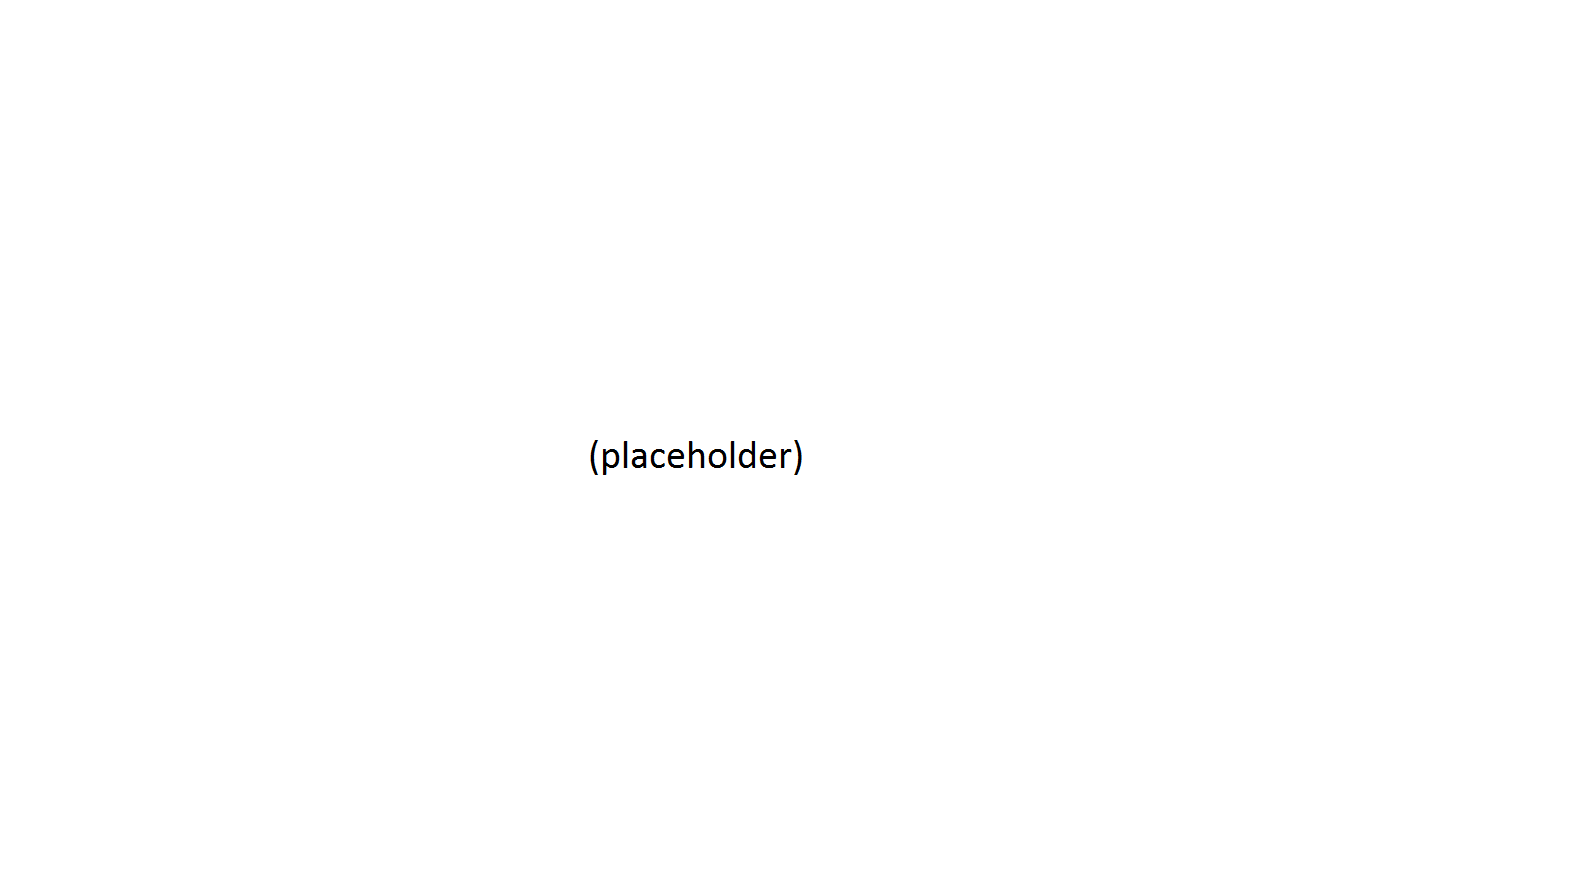
\includegraphics[width=.45\linewidth]{./fig/mc_theta.png}
% \label{fig:mctheta}}
% \quad
% \subfigure[Reconstructed]{%
% 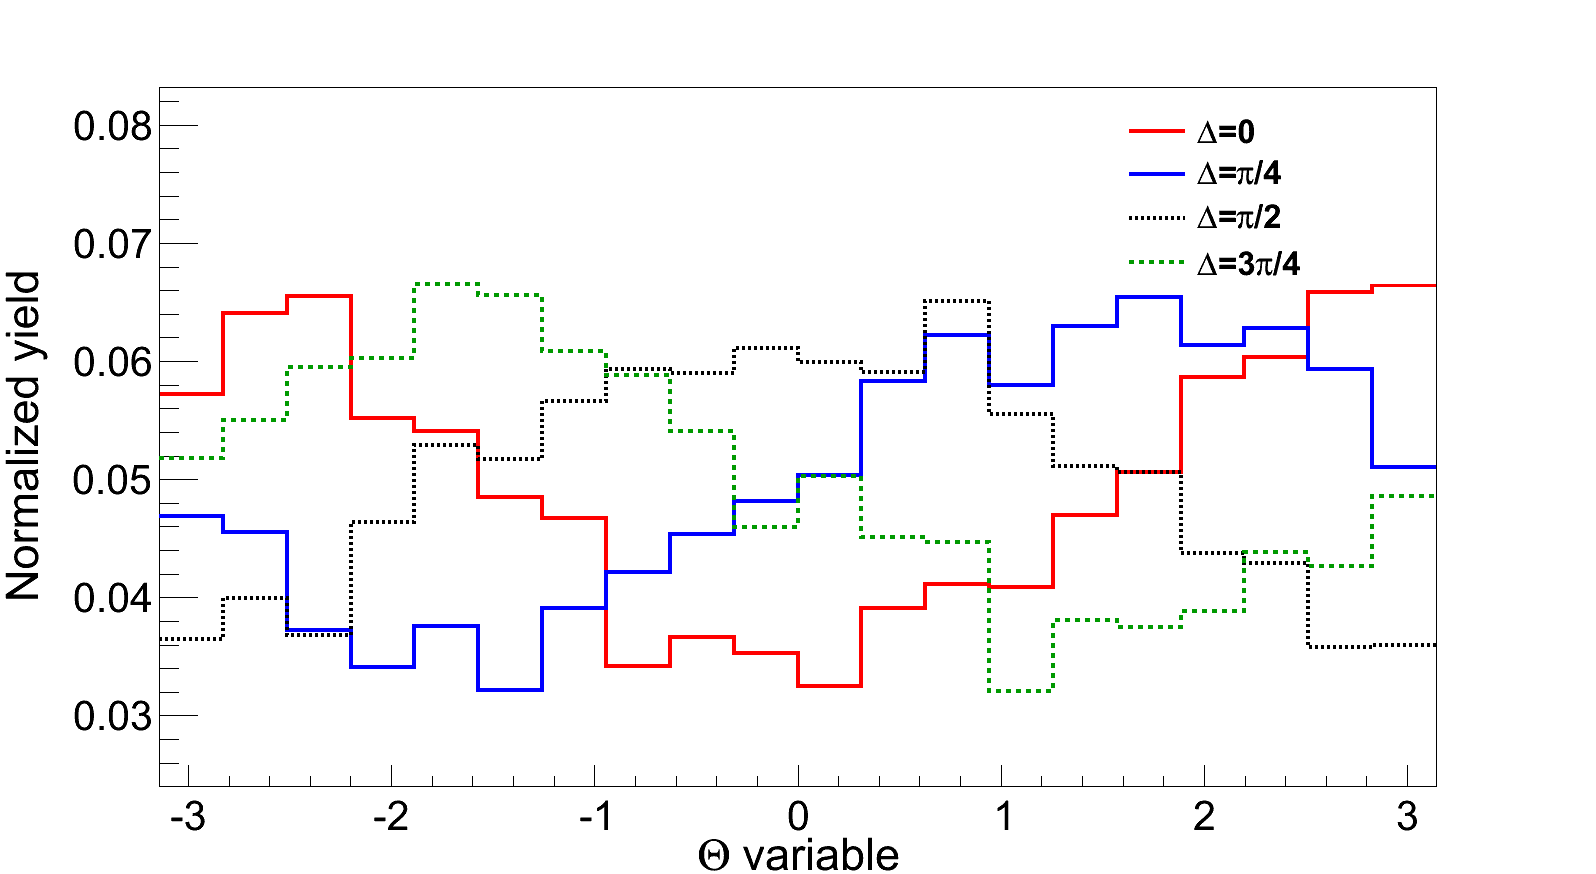
\includegraphics[width=.45\linewidth]{./fig/reco_theta.png}
% \label{fig:recotheta}}
% \caption{Comparison of $\Theta$ variable distribution between generated and reconstructed information for various values of the phase $\Delta$. Although the amplitude of the oscillation is decreased, the overall shape is preserved.}
% \label{fig:thetaResult}
% \end{figure}

% From the maximum likelihood method we obtain an uncertainty on the measurement of $59^\circ$ for a dataset of 1 ab$^{-1}$. This is much worse than the $4.4^\circ$ uncertainty obtained by Ref.~\cite{harnik}. Thus, we see that detector effects play an important role in this measurement and cannot be neglected.

%%%%%%%%%%%%%%%%%%%%%%%%%%%%%%%%%%%%%%%%%%%%%%
\section{Conclusion}
\label{sec:conclusion}


This will be the conclusion.

% We have shown that detector effects, which were neglected by previous studies, play an important role in this measurement. The main obstacle is to accurately reconstruct the $Z$ 4-momentum. This can only be done for leptonic $Z$ decays, which results in a very decreased signal yield culminating in a very limited accuracy of the measurement.

\clearpage

% %%%%%%%%%%%%%%%%%%%%%%%%%%%%%%%%%%%%%%%%%%%%%%
% \begin{thebibliography}{99}

% \bibitem{higgs}
%  P.~W.~Higgs,
%   %``Broken symmetries, massless particles and gauge fields,''
%   Phys.\ Lett.\  {\bf 12}, 132 (1964);
%   %%CITATION = PHLTA,12,132;%%
%  P.~W.~Higgs,
%   %``BROKEN SYMMETRIES AND THE MASSES OF GAUGE BOSONS,''
%   Phys.\ Rev.\ Lett.\  {\bf 13}, 508 (1964);
%   %%CITATION = PRLTA,13,508;%%
%  F.~Englert and R.~Brout,
%   %``BROKEN SYMMETRY AND THE MASS OF GAUGE VECTOR MESONS,''
%   Phys.\ Rev.\ Lett.\  {\bf 13}, 321 (1964).
%   %%CITATION = PRLTA,13,321;%%

% \bibitem{discovery}
%   G.~Aad {\it et al.} [ATLAS Collaboration],
%   %% July 12 discovery paper
%   Phys.\ Lett.\ B {\bf 716}, 1 (2012),
%   %[arXiv:1207.7214 [hep-ex]]
%   S.~Chatrchyan {\it et al.}  [CMS Collaboration],
%   %% July 12 discovery paper
%   Phys.\ Lett.\ B {\bf 716}, 30 (2012).
%   %[arXiv:1207.7235 [hep-ex]].
  
% \bibitem{atlas_cp1}
%   G.~Aad {\it et al.} [ATLAS Collaboration],
%   Eur. Phys. J. {\bf C75} (2015) 476.
%   %[arXiv:1506.05669v2]
  
% \bibitem{cms_cp}
%   S.~Chatrchyan {\it et al.}  [CMS Collaboration],
%   Phys. Rev. Lett. {\bf 110} (2013) 081803
%   %[arXiv:1212.6639v2]
  
% \bibitem{atlas_cp2}
%   G.~Aad {\it et al.} [ATLAS Collaboration],
%   	CERN-EP-2016-002.
%   	%[arXiv:1602.04516v1]
  
% \bibitem{harnik}
%   R.~Harnik {\it et al.},
%   Phys. Rev. D {\bf 88}, 076009 (2013)
%   %[arXiv:1308.1094v1]
  
% \bibitem{worek}
%   M.~Worek,
%   Acta Phys.Polon. {\bf B34} (2003) 5531-5538
%   %[hep-ph/0310205]
  
% \bibitem{berge}
%   S.~Berge, W.~Bernreuther, and H.~Spiesberg,
%   Phys. Lett. {\bf B727}, 488 (2013), 1308.2674
%   %[arXiv:1308.1094v1]
  
% \bibitem{ilc}
%   Linear Collider Collaboration, ILC Technical Design Report, \url{http://www.linearcollider.org/ILC/Publications/Technical-Design-Report}
  
% \bibitem{fccee}
%   CERN, The FCC-ee design study, \url{http://tlep.web.cern.ch/}
  
% \bibitem{madgraph}
%   J.~Alwall {\it et al.},
%   {\it JHEP} {\bf 07} (2014) 079.
%   %[arXiv:1405.0301v2]
  
% \bibitem{pythia}
%   T.~Sjostrand, S.~Mrenna, and P.Z.~Skands,
%   Comput. Phys. Commun. {\bf 178} (2008) 852–867.
%   %[arXiv:0710.3820v1]
 
% \bibitem{delphes}
%   J.~de~Favereau {\it et al.} [DELPHES 3 collaboration],
%   {\it JHEP} {\bf 02} (2014) 057.
%   %[arXiv:1307.6346v3]
  
% \bibitem{cacciari}
%   M.~Cacciari, G.~Salam, G.~Soyez,
%   {\it JHEP} {\bf 04}, 063 (2008), 0802.1189.
%   %[arXiv:0802.1189]
  
% \end{thebibliography}

\end{document} 
